\documentclass[usenames,dvipsnames,french]{beamer}

\mode<presentation> {

\usetheme{Montpellier}
}

\usepackage{graphicx} % Allows including images
\usepackage[frenchb]{babel}
\usepackage[T1]{fontenc}
\usepackage[utf8]{inputenc}
% \usepackage[demo]{graphicx}
% \usepackage{caption}

\usepackage{subcaption}
% \usepackage{subfig}
% \usepackage{algorithm,algorithmic}
\usepackage{algorithm2e}
\usepackage{listings}
% \usepackage{ntheorem}
\usepackage{booktabs} % Allows the use of \toprule, \midrule and \bottomrule in tables
\setcounter{tocdepth}{2}
\graphicspath{{../../Figures/}}


\DeclareMathOperator*{\argmin}{arg\,min}
\DeclareMathOperator*{\argmax}{arg\,max}
\newtheorem*{proposition}{Proposition}

% exercices comptés
\newcounter{numexos}%Création d'un compteur qui s'appelle numexos
\setcounter{numexos}{0}%initialisation du compteur
\newcommand{\exercice}[1]{%Création d'une macro ayant un paramètre
\addtocounter{numexos}{1}%chaque fois que cette macro est appelée, elle ajoute 1 au compteur numexos
\textcolor{DarkOrchid}{Exercice\,\thenumexos\,:}\,#1%Met en rouge Exercice et la valeur du compteur appelée par \thenumeexos
}
%----------------------------------------------------------------------------------------
%	TITLE PAGE
%----------------------------------------------------------------------------------------

\setbeamertemplate{title page}{
    \centering

    \Large\bfseries
    Machine Learning Tek 5: train and test set, regression.
    

\begin{figure}[!h]
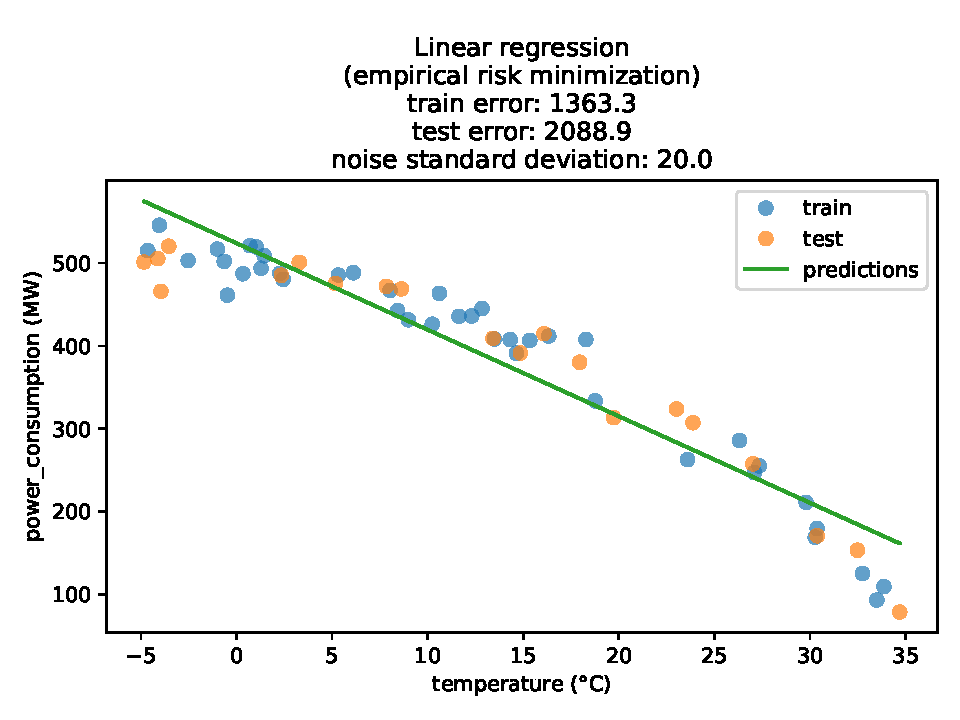
\includegraphics[width=8cm]{optimal_linear_regression_standard_deviation_20_0}
\end{figure}

    }
\begin{document}

\frame{\titlepage}

\begin{frame}{Content}

    \tableofcontents

\end{frame}

\section*{Introduction}

\begin{frame}{Linear regression}

    Linear regression is one of the most elementary methods used in ML
    regression problems. It is useful for many applications, and is often a
    component of more complex methods.

    We will use is to illustrate several important aspects of ML that are also
    encountered when using other methods (kernels, trees, neural networks, etc.), namely:
    \begin{itemize}
    	\item the train and test sets.
	\item overfitting (when the dimension $d$ is not really small).
    \end{itemize}

\end{frame}

\section{Train sets and test sets, loss functions}%
\label{sec:Train sets and test sets}

\begin{frame}{Example problem}

    We want to predict the power that needs to be produced by a power plant in
    a city, as a function of the temperature only.

    \begin{figure}[htpb]
        \centering
        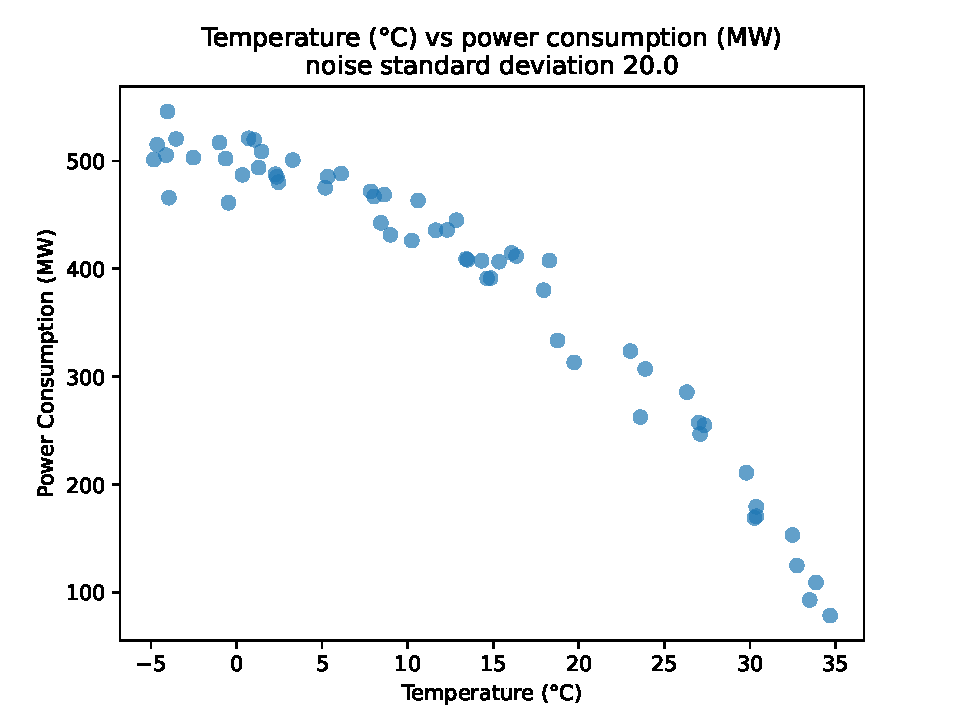
\includegraphics[width=0.6\textwidth]{dataset_standard_deviation_20_0}
        \caption{Dataset}
        \label{fig:dataset}
    \end{figure}
\end{frame}

\begin{frame}

    The only information we have is a collection of $n$ \textbf{samples}, called the \textbf{dataset}. Each sample consists in two values:

    \begin{itemize}
	\item the temperature in °C (the \textbf{feature}).
	\item the power consumption in W (the \textbf{label}).
    \end{itemize}

    \begin{figure}[htpb]
        \centering
        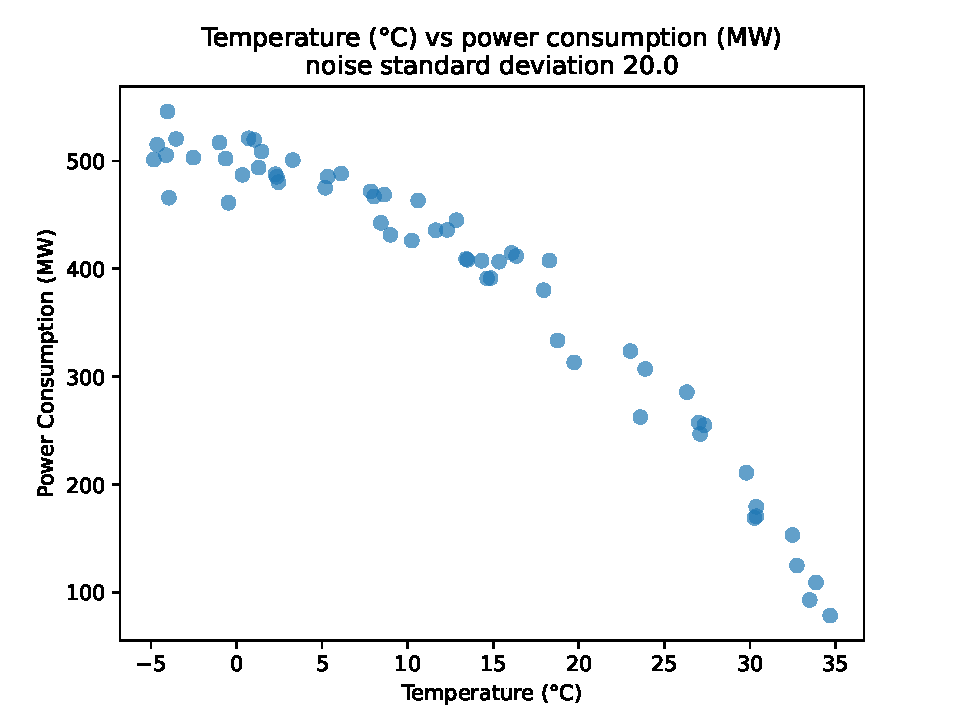
\includegraphics[width=0.4\textwidth]{dataset_standard_deviation_20_0}
        \caption{Dataset}
        \label{fig:dataset}
    \end{figure}
    \exercice{} What is $d$ in this example ?
\end{frame}

\begin{frame}{Supervised learning}

    Based on this \textbf{finite} dataset, our objective is to produce a function, noted $\tilde{f}$, called the \textbf{model}, the \textbf{predictor}, or the \textbf{estimator}, that will map a temperature to a power consumption.

    \begin{figure}[htpb]
        \centering
        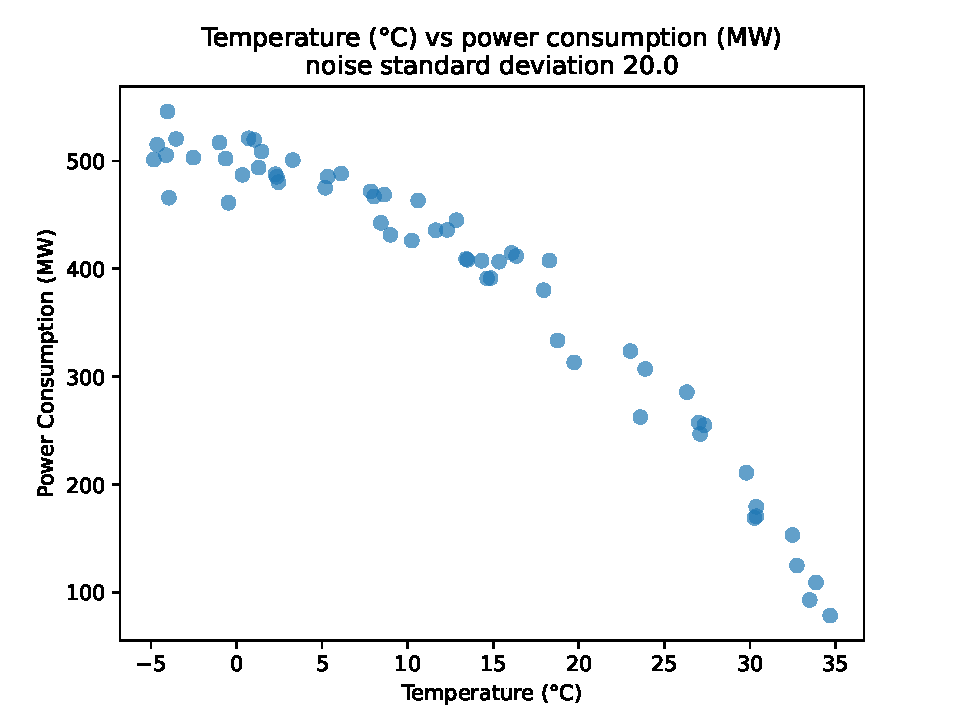
\includegraphics[width=0.3\textwidth]{dataset_standard_deviation_20_0}
        \caption{Dataset}
        \label{fig:dataset}
    \end{figure}

    The problem of supervised learning is that we want this function to perform well on \textbf{new, previously unseen samples}. It is not useful in itsself to perform well on the dataset !

\end{frame}

\begin{frame}{Supervised learning}

    Based on this \textbf{finite} dataset, our objective is to produce a function, noted $\tilde{f}$, that will map a temperature to a power consumption.

    \begin{figure}[htpb]
        \centering
        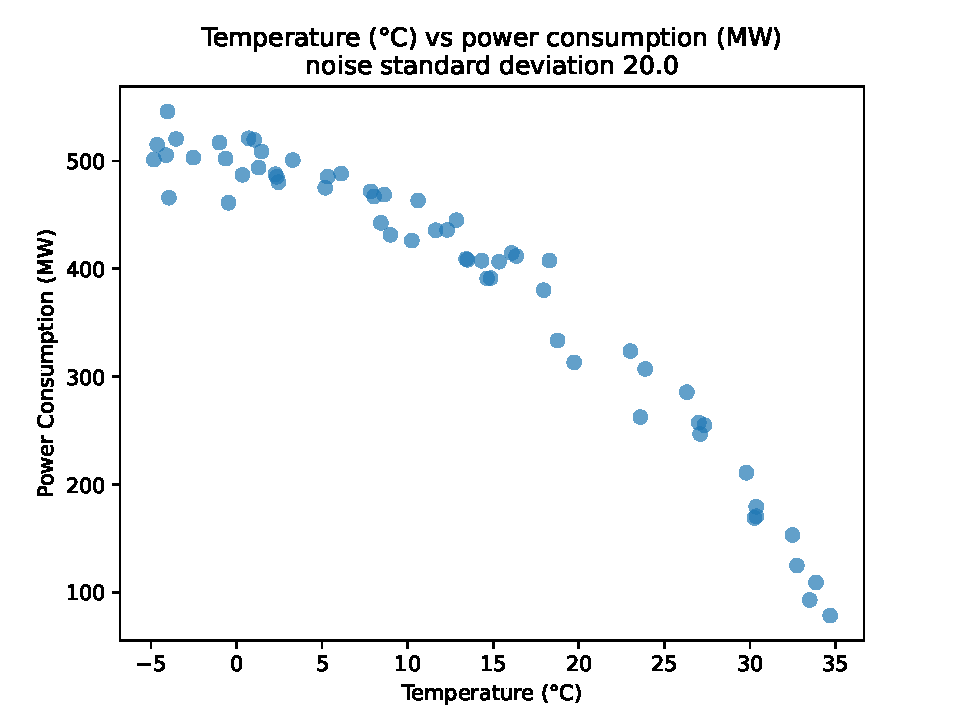
\includegraphics[width=0.3\textwidth]{dataset_standard_deviation_20_0}
        \caption{Dataset}
        \label{fig:dataset}
    \end{figure}

    \exercice{} How could we \textbf{estimate} the performance of $\tilde{f}$ on unseen data, using the dataset ?
    
\end{frame}

\begin{frame}{Train set and set set}
    We split the dataset in two parts:
    \begin{itemize}
	\item the \textbf{train set} will be used to learn (train $\tilde{f}$)
	\item the \textbf{test set} will be used to estimate the performance of $\tilde{f}$ on unseen data.
    \end{itemize}
    \begin{figure}[htpb]
        \centering
        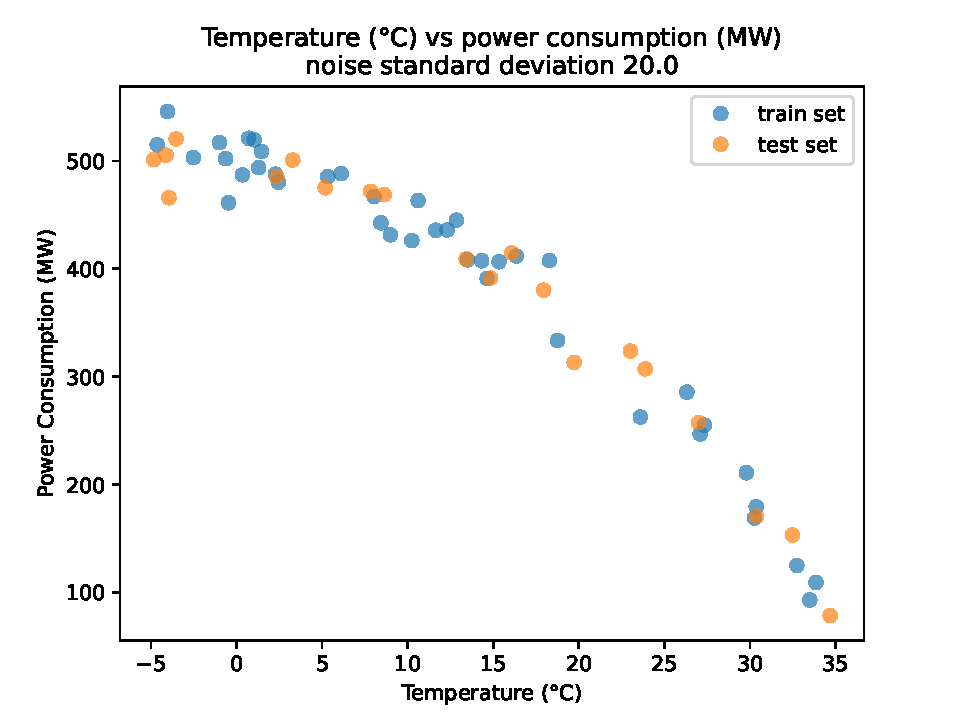
\includegraphics[width=0.5\textwidth]{dataset_standard_deviation_20_0_splitted}
        \caption{Splitted Dataset}
        \label{fig:dataset}
    \end{figure}
\end{frame}

\begin{frame}{Loss functions}

    To evaluate the performance of $\tilde{f}$, we use a \textbf{loss function}. The loss function is be a measure of the \textbf{discrepancy} between a prediction $\tilde{f}(x)$ and a \text{label} $y$ (that are both real numbers). In regression, the most common loss function is the squared loss:
	    \begin{equation}
		(\tilde{f}(x)-y)^2
	    \end{equation}

	 Averaging over the whole dataset, this leads to:
	 \begin{itemize}
	     \item The train error
	    \begin{equation}
		\frac{1}{n_{\text{train}}}\sum_{(x_i, y_i)\in (X_{train}\times y_{train})} (\tilde{f}(x_i)-y_i)^2
	    \end{equation}
	     \item The test error
	    \begin{equation}
		\frac{1}{n_{\text{test}}}\sum_{(x_i, y_i)\in (X_{test}\times y_{test})} (\tilde{f}(x_i)-y_i)^2
	    \end{equation}
	 \end{itemize}
\end{frame}

\begin{frame}{Empirical risk minimization}

    The most common supervised learning process is then naturally to:
    \begin{itemize}
    	\item Find $\tilde{f}$ the as a small training error.
	\item Compute the test error of $\tilde{f}$ in order to estimate its performance on unseen data.
    \end{itemize}

    \textbf{Remark}: many of these two aspects will be discussed more deeply later in the couse (e.g. notions of validation set, or optimization error)
\end{frame}

\section{Linear regression in one dimension}
\frame{\tableofcontents[currentsection]}

\begin{frame}{Linear regression}

    The remaining step is then to find $\tilde{f}$. The first step, called \textbf{model selection}, is to decide the type of function / model use. Many types of models exist, each one having potential drawbacks, for instance:
    \begin{itemize}
	\item linear functions (which we will use in this first example).
	\item polynomial functions
	\item kernels
	\item neural networks
	\item support vector machines
    \end{itemize}

    \url{https://scikit-learn.org/stable/machine_learning_map.html} 

\end{frame}


\begin{frame}{}

    \exercice{} Why are the samples not on a line (and not on a curved line either) ?

    \begin{figure}[htpb]
        \centering
        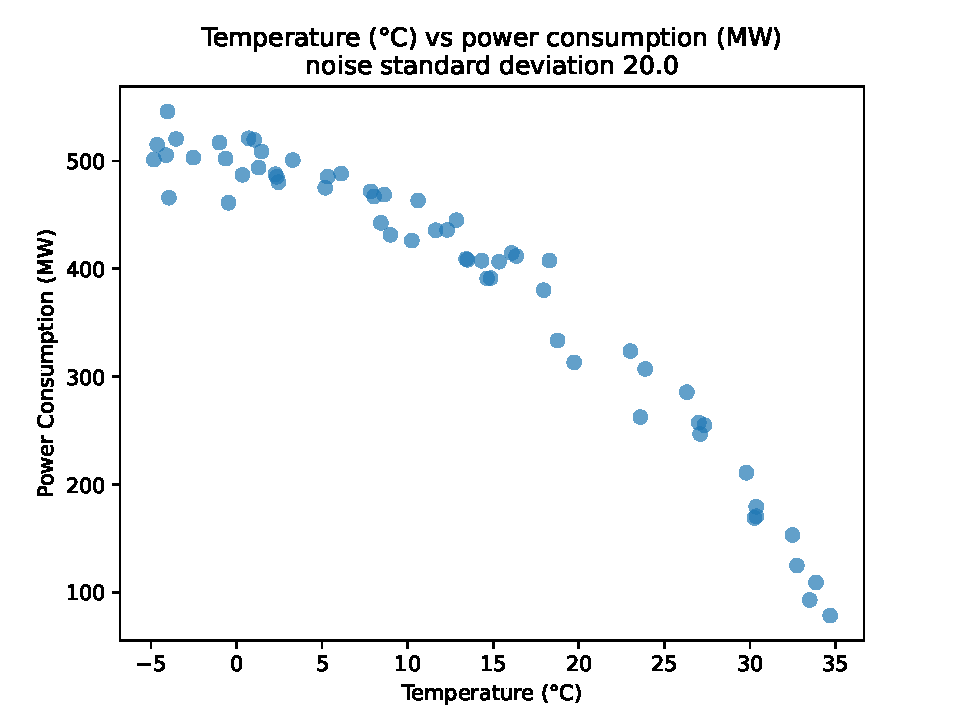
\includegraphics[width=0.6\textwidth]{dataset_standard_deviation_20_0}
        \caption{Dataset}
        \label{fig:dataset}
    \end{figure}

\end{frame}

\begin{frame}{}

    \begin{figure}[htpb]
        \centering
        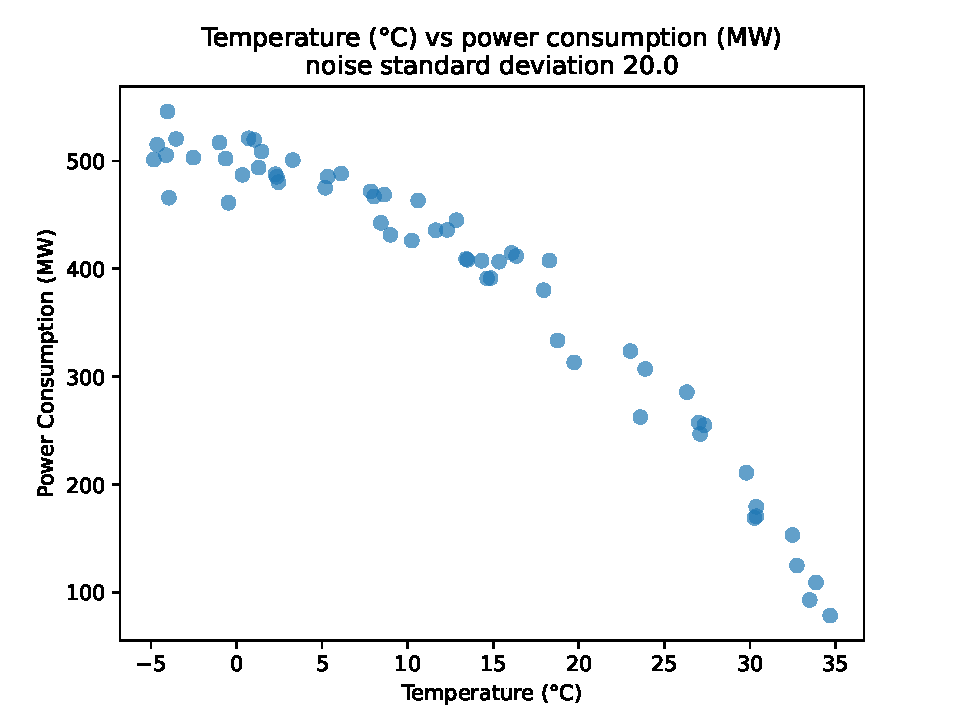
\includegraphics[width=0.3\textwidth]{dataset_standard_deviation_20_0}
        \caption{Dataset}
        \label{fig:dataset}
    \end{figure}

    The power consumption does not depend \textbf{only} on the temperature,
    but also on many other variables, that we do not have access to here:
    \begin{itemize}
        \item time in the day
        \item humidity, wind
        \item period of the year (holidays or not)
        \item other variables
    \end{itemize}

\end{frame}

\begin{frame}{Linear regression}

    Formalization:
    \begin{itemize}
        \item input space (temperature in °C): $\mathcal{X} = \mathbb{R}$
        \item output space (power consumption in W): $ \mathcal{Y} = \mathbb{R}$
	\item dataset: $D=\{(x_1, y_1), \dots, (x_n, y_n), i\in[1, n]\}$.
    \end{itemize}

    \textbf{linear regression} in dimension $1$ (as $x\in \mathbb{R}$), means that our estimator is of the form:

    \begin{equation}
        \tilde{f}(x) = \theta x + b
    \end{equation}

    with $\theta\in \mathbb{R}$, $b\in \mathbb{R}$.

\end{frame}

\begin{frame}{Empirical risk minimization}

    With the squared loss, and this function $ \tilde{f}$ the \textbf{train error} is:

    \begin{equation}
	R_{n_{train}}(\theta, b) = \frac{1}{n_{train}} \sum_{(x_i, y_i)\in (X_{train}\times y_{train})} (\theta x_i+b-y_i)^2
    \end{equation}

    The \textbf{optimization problem} is to find $\theta$ and $b$ such that $R_{n_{train}}(\theta, b)$ has the
    \textbf{smallest possible value}. 
\end{frame}

\begin{frame}{Numpy}

    Numpy demo.

\end{frame}

\begin{frame}

    \exercice{}

    \textbf{cd code/day\textunderscore 1/1\textunderscore linear\textunderscore regression /1D\textunderscore linear\textunderscore regression/}

    \begin{itemize}
    	\item Generate some data using \textbf{main\textunderscore create\textunderscore data.py}. You can choose the amplitude of the noise by setting STD\textunderscore NOISE in \textbf{constants.py} (we will discuss the importance of this constant shortly). The images are generated in the \textbf{images/datasets/} folder.
    \item fix \textbf{utils.py} in order to correctly compute the train error and test error.
    \end{itemize}

    Launch \textbf{main\textunderscore random\textunderscore params.py} in order to test several values for $\theta$ and $b$ by evaluating their empirical risk. Note that you can know whether your result is correct thanks to the ground truth (mse()).

    \textbf{Remark:} In VSCode, you need to execute the python script from the correct location (namely from \textbf{1D\textunderscore linear\textunderscore regression}) in order for the paths to properly work.

\end{frame}

\begin{frame}{Analytic solutions}

    For some problems, like this one, it is possible to explicitely compute the
    optimal solution.
    \\

    For some advanced reasons (convexity and differentiability of
    $R_n(\theta)$), the points optimizing the empirical risk are obtained by
    finding $ (\theta^*, b^*)$ such that the gradient cancels (more on that
    later in the course).

    \begin{equation}
        \nabla_{(\theta, b)} R_n(\theta^*, b^*) = 0
    \end{equation}
\end{frame}

\begin{frame}{Derivatives}
    We drop the  $\frac{1}{n}$ as it does not change the final result:
    \begin{equation}
    \begin{aligned}
        \label{eq:}
        \frac{\partial R_n}{\partial \theta}(\theta, b) &= \sum_{i=1}^{n} 2(\theta x_i+b-y_i)x_i\\
        &= 2\Large[\theta \sum_{i=1}^{n} x_i^2 + b\sum_{i=1}^{n} x_i - \sum_{i=1}^{n} x_i y_i \Large]\\
    \end{aligned}
    \end{equation}


    \begin{equation}
    \begin{aligned}
        \label{eq:}
        \frac{\partial R_n}{\partial b}(\theta, b) &= \sum_{i=1}^{n} 2(\theta x_i+b-y_i)\\
        &= 2\Large[\theta \sum_{i=1}^{n} x_i + nb- \sum_{i=1}^{n} y_i \Large]\\
    \end{aligned}
    \end{equation}
\end{frame}

\begin{frame}{}
    Hence we have a system of $2$ equations with $2$ unknowns (dropping the $\theta^*$ notation)

    \begin{equation}
        \theta \sum_{i=1}^{n} x_i^2 + b\sum_{i=1}^{n} x_i - \sum_{i=1}^{n} x_i y_i = 0
    \end{equation}

    \begin{equation}
        \theta \sum_{i=1}^{n} x_i + nb- \sum_{i=1}^{n} y_i = 0
    \end{equation}
\end{frame}

\begin{frame}{}
    Which means

    \begin{equation}
        b =  \frac{1}{n}(\sum_{i=1}^{n} y_i -\theta \sum_{i=1}^{n} x_i)
    \end{equation}

    \begin{equation}
        \theta \sum_{i=1}^{n} x_i^2 + \frac{1}{n}\large(\sum_{i=1}^{n} y_i -\theta \sum_{i=1}^{n} x_i \large)\sum_{i=1}^{n} x_i - \sum_{i=1}^{n} x_i y_i = 0
    \end{equation}

\end{frame}

\begin{frame}
    Finally:

    \begin{equation}
        \theta (\sum_{i=1}^{n} x_i^2 - \frac{1}{n}(\sum_{i=1}^{n} x_i)^2) +\frac{1}{n}\sum_{i=1}^{n} x_i\sum_{i=1}^{n} y_i - \sum_{i=1}^{n} x_i y_i = 0
    \end{equation}

    or

    \begin{equation}
        \theta^* = \frac{\sum_{i=1}^{n} x_i y_i - \frac{1}{n}\sum_{i=1}^{n} x_i\sum_{i=1}^{n} y_i}{\sum_{i=1}^{n} x_i^2 - \frac{1}{n}[\sum_{i=1}^{n} x_i]^2}
    \end{equation}
\end{frame}


\begin{frame}{}

    \exercice{}

    Fix \textbf{main\textunderscore optimal\textunderscore params.py} in order to plot the linear
    regression found with the analytic solution on the same plot as the raw
    dataset.

    \begin{figure}[htpb]
        \centering
        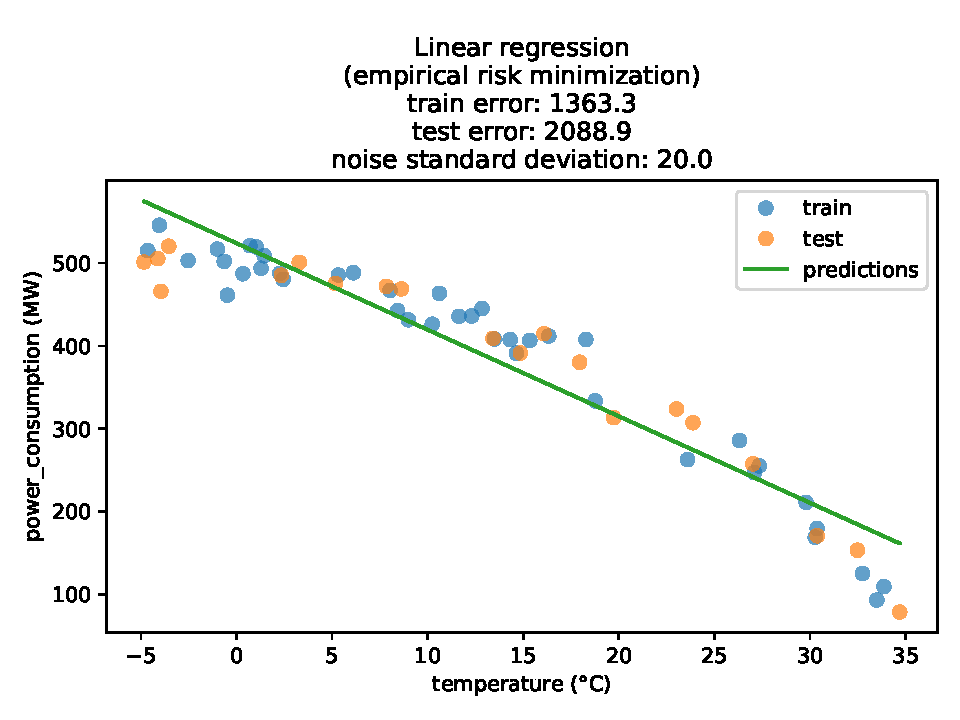
\includegraphics[width=0.7\textwidth]{optimal_linear_regression_standard_deviation_20_0}
        \label{fig:dataset_with_regression}
    \end{figure}

\end{frame}

\begin{frame}{Scikit}

    With \textbf{main\textunderscore scikit.py}, we can perform the same computation using scikit, and verify that the obtained estimator is identical.

\end{frame}

\section{Polynomial regression and overfitting}%
\label{sec:Polynomial regression and overfitting}

\begin{frame}{Different model ?}
    \exercice{} Could we use a better \textbf{model} for this dataset ?
    \begin{figure}[htpb]
        \centering
        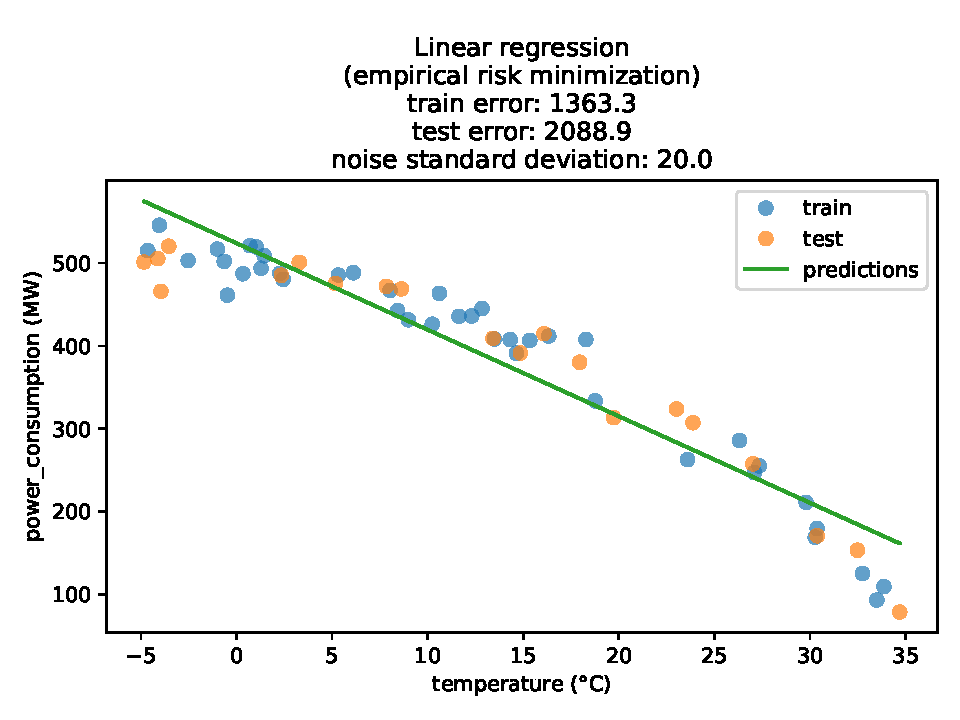
\includegraphics[width=0.7\textwidth]{optimal_linear_regression_standard_deviation_20_0}
        \label{fig:dataset_with_regression}
    \end{figure}
\end{frame}

\begin{frame}
    Instead of a linear predictor, we could use a polynom. If $t$ is the temperature, the polynomial predictor writes:
    \begin{equation}
	\tilde{f}(t) = a_0 + a_1 t + a_2 t^2 + \dots + a_d t^d
    \end{equation}
    with the \textbf{degree} $d$ being a constant to determine.
    \begin{figure}[htpb]
        \centering
        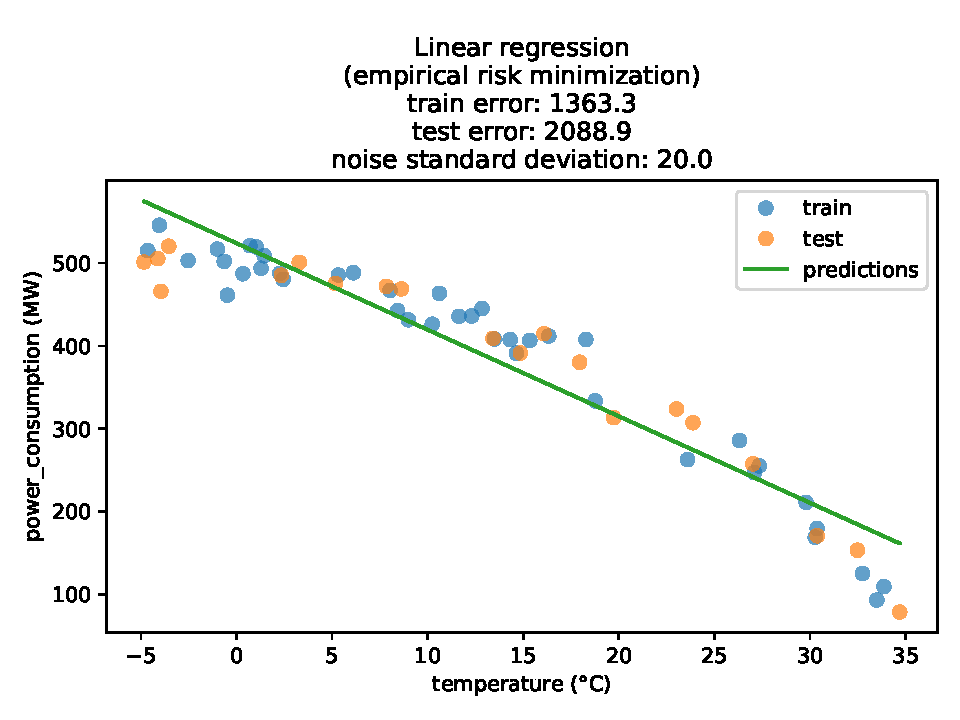
\includegraphics[width=0.4\textwidth]{optimal_linear_regression_standard_deviation_20_0}
        \label{fig:dataset_with_regression}
    \end{figure}
\end{frame}

\begin{frame}{Fitting polynomials}

    Using \textbf{main\textunderscore polynomial\textunderscore regression.py}, in which the optimization problem is directly handeled by numpy, we will make several observations.

    \begin{figure}[htpb]
    	\centering
    	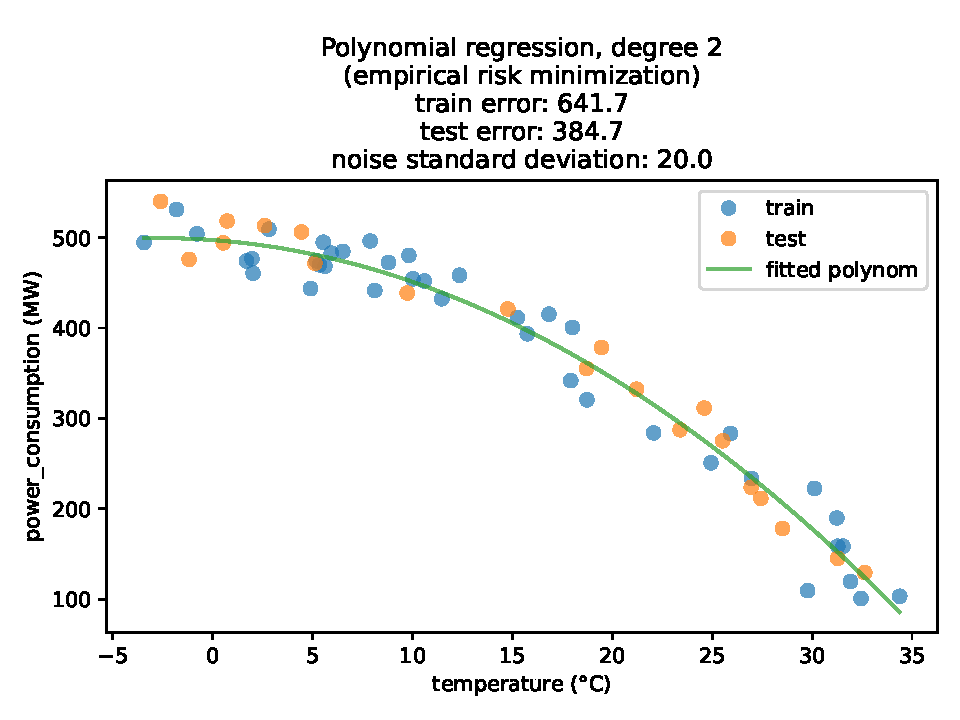
\includegraphics[width=0.7\textwidth]{polyomial_regression_std_20_0_degree_2}
    	\label{fig:}
    \end{figure}

\end{frame}

\begin{frame}

    The test error is smaller with this polynomial fit of degree $2$ than for the linear regression.

    \begin{figure}[htpb]
    	\centering
    	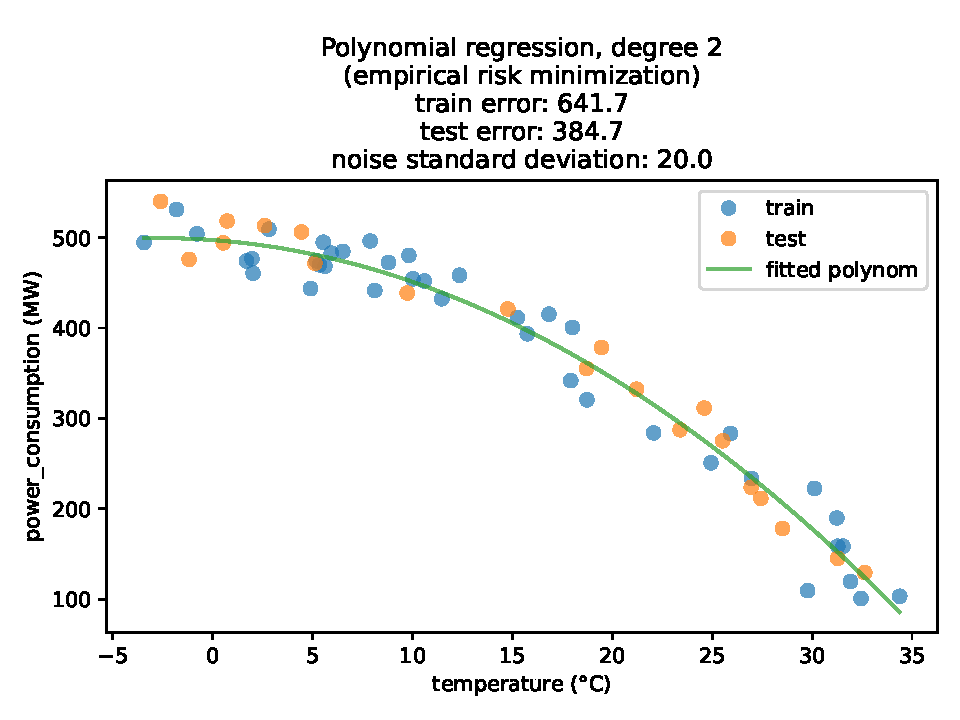
\includegraphics[width=0.7\textwidth]{polyomial_regression_std_20_0_degree_2}
    	\label{fig:}
    \end{figure}

\end{frame}


\begin{frame}

    If the degree of the polynom is too large, \textbf{overfitting} happens.

    \begin{figure}[htpb]
    	\centering
    	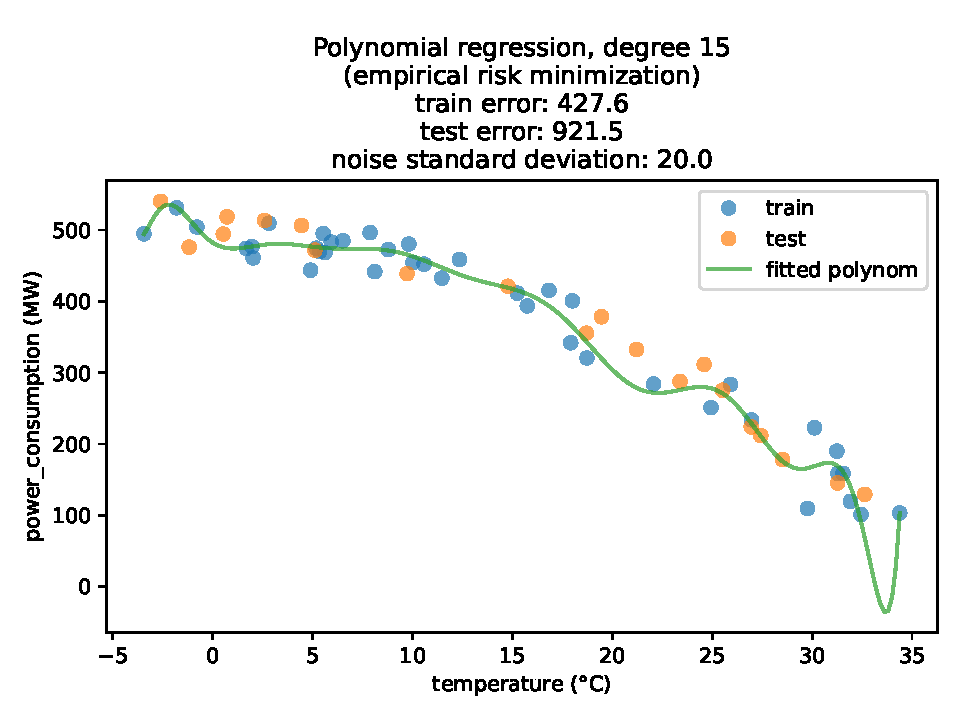
\includegraphics[width=0.7\textwidth]{polyomial_regression_std_20_0_degree_15}
    	\label{fig:}
    \end{figure}

\end{frame}


\begin{frame}

    If the degree of the polynom is too large, \textbf{overfitting} happens.

    \begin{figure}[htpb]
    	\centering
    	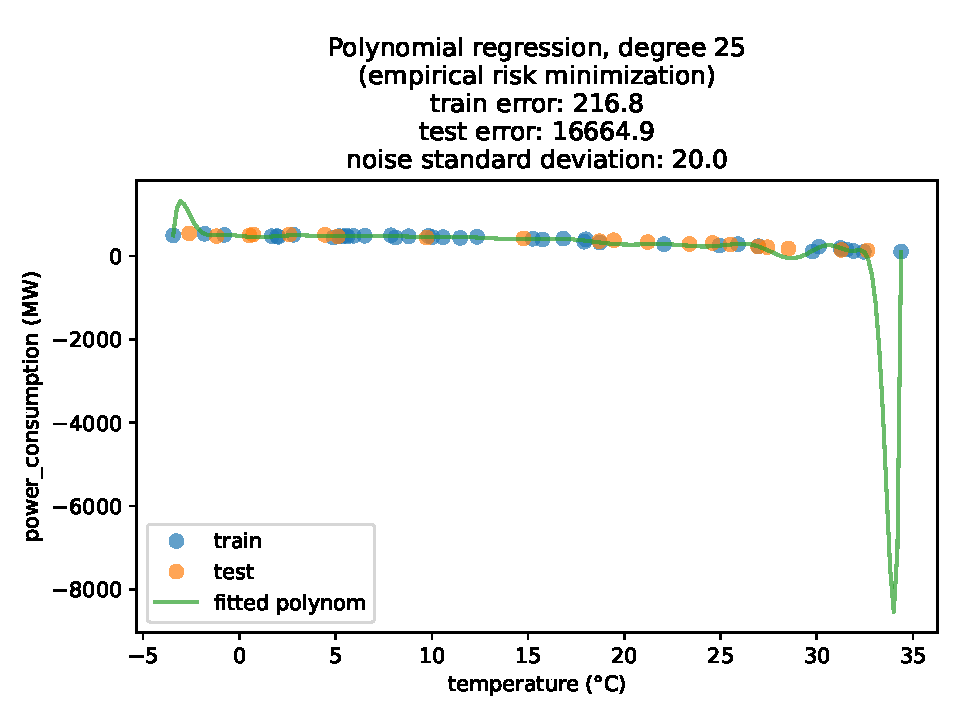
\includegraphics[width=0.7\textwidth]{polyomial_regression_std_20_0_degree_25}
    	\label{fig:}
    \end{figure}

\end{frame}


\begin{frame}

    If the degree of the polynom is too large, \textbf{overfitting} happens.

    \begin{figure}[htpb]
    	\centering
    	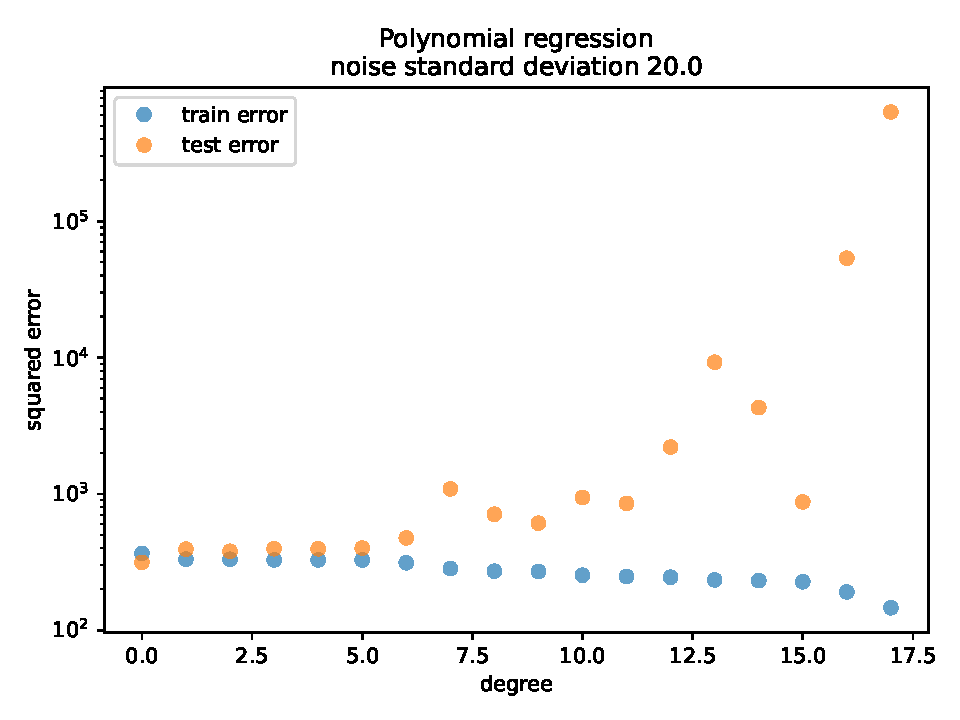
\includegraphics[width=0.7\textwidth]{polynomial_regression_standard_deviation_20_0}
    	\label{fig:}
    \end{figure}

\end{frame}

\begin{frame}

    Reducing the noise standard deviation reduces overfitting

    \begin{figure}[htpb]
    	\centering
    	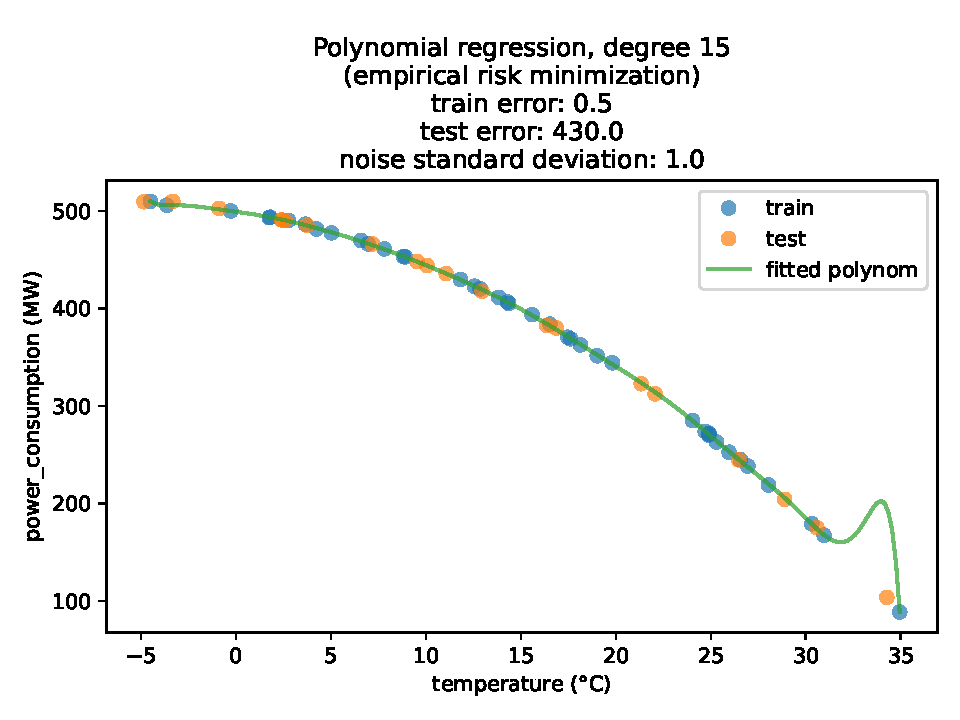
\includegraphics[width=0.7\textwidth]{polyomial_regression_std_1_0_degree_15}
    	\label{fig:}
    \end{figure}

\end{frame}


\begin{frame}

    Reducing the noise standard deviation reduces overfitting

    \begin{figure}[htpb]
    	\centering
    	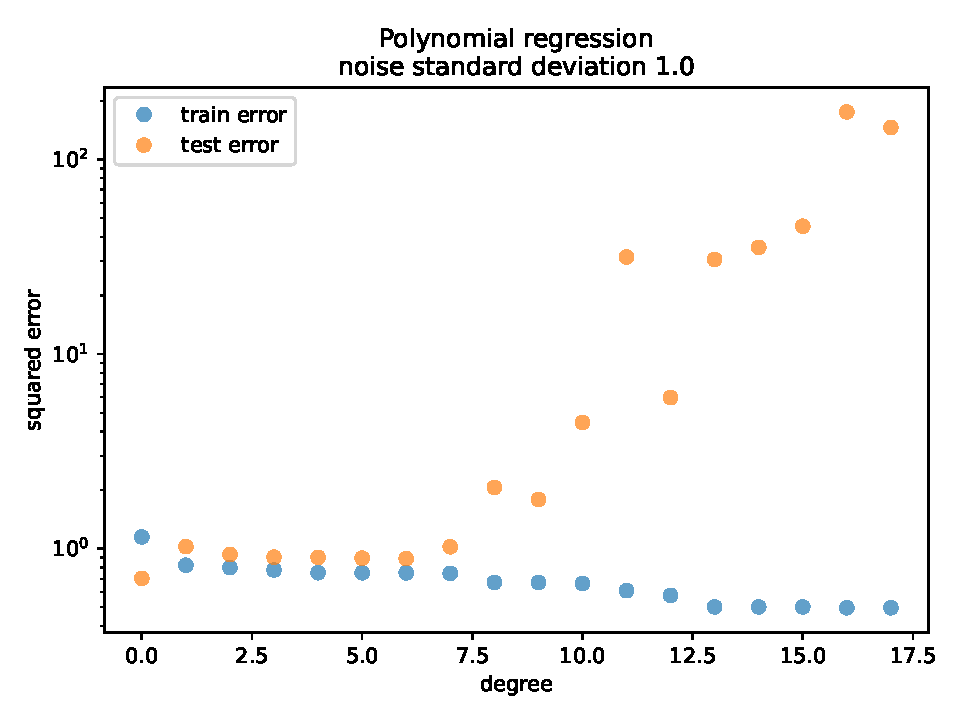
\includegraphics[width=0.7\textwidth]{polynomial_regression_standard_deviation_1_0}
    	\label{fig:}
    \end{figure}

\end{frame}


\begin{frame}

    If there is no noise, there is no overfitting !

    \begin{figure}[htpb]
    	\centering
    	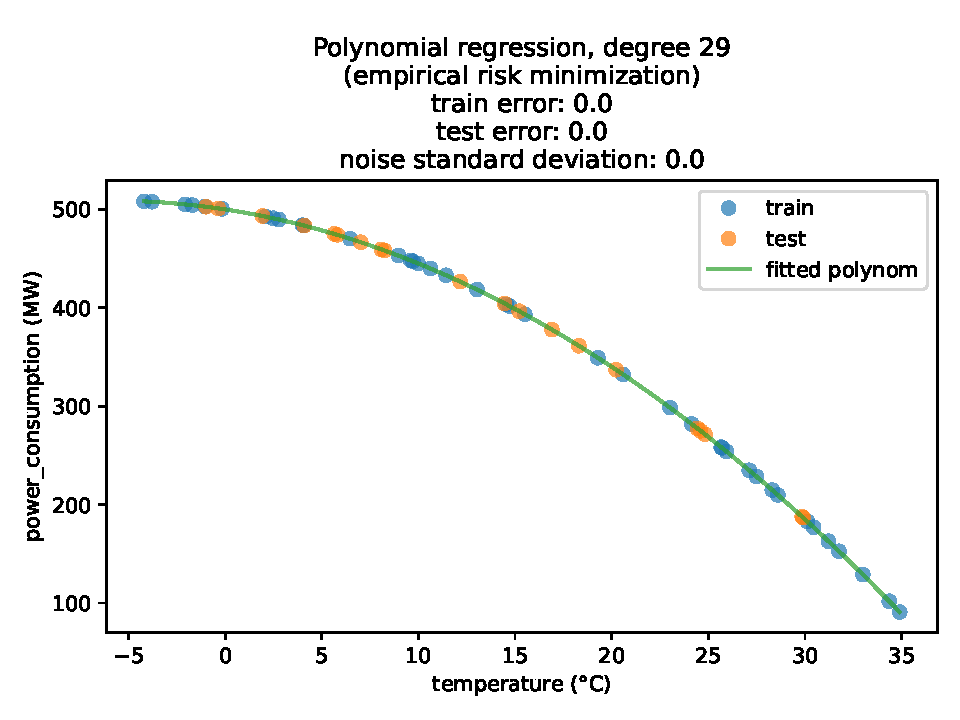
\includegraphics[width=0.7\textwidth]{polyomial_regression_std_0_0_degree_29}
    	\label{fig:}
    \end{figure}

\end{frame}



\begin{frame}

    If there is no noise, there is no overfitting !

    \begin{figure}[htpb]
    	\centering
    	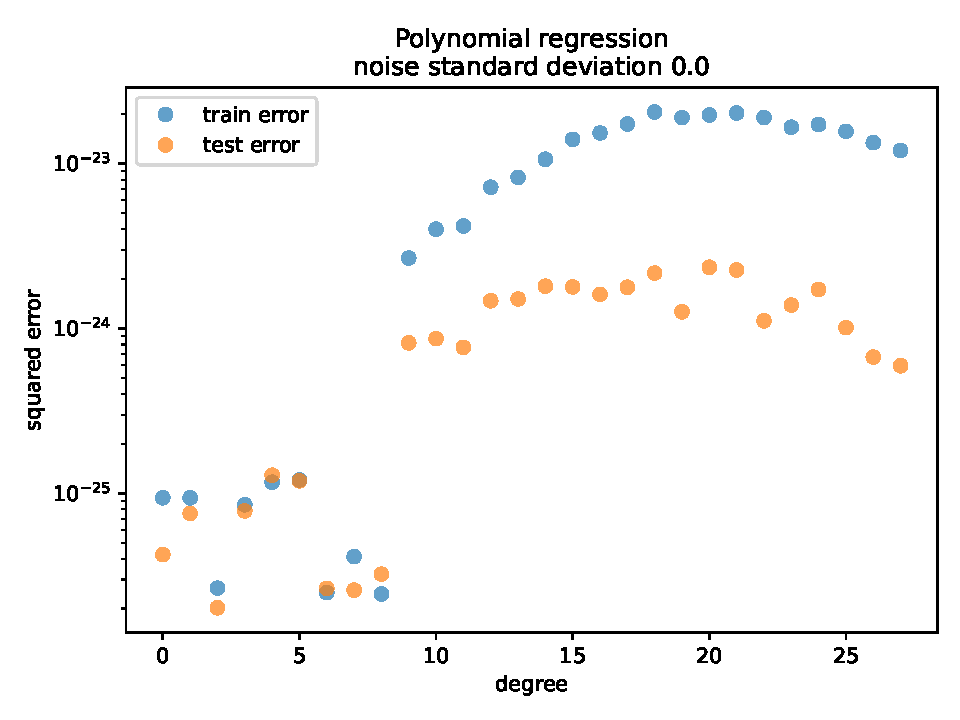
\includegraphics[width=0.7\textwidth]{polynomial_regression_standard_deviation_0_0}
    	\label{fig:}
    \end{figure}

\end{frame}

\begin{frame}

    Having more samples also reduces overfitting.

    \begin{figure}[htpb]
    	\centering
    	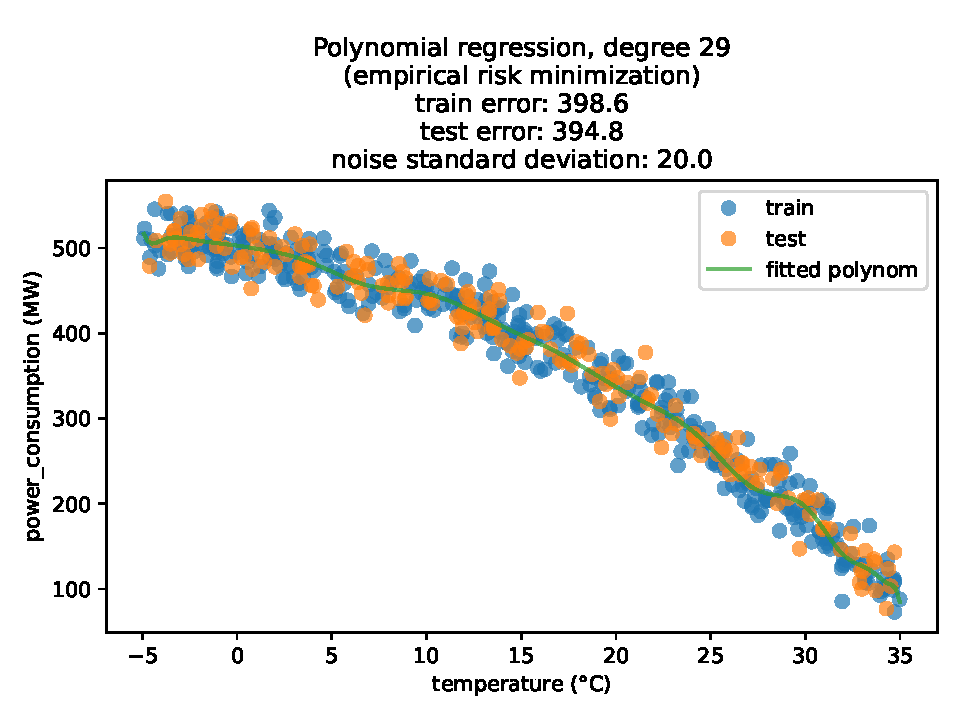
\includegraphics[width=0.7\textwidth]{polyomial_regression_std_20_0_degree_29_more_samples}
    	\label{fig:}
    \end{figure}

\end{frame}

\begin{frame}{Conclusion}

    The amount of overfitting depend on the \textbf{balance} between:
    \begin{itemize}
    	\item the number of parameters / features / dimension $d$ of the problem
	\item the number of available samples
    \end{itemize}

    Neural networks show some specific behavior on that topic, that we will study later.

    \textbf{Important remark}: most of the time, it is not possible to have such a direct \textbf{visualisation} of the data (as soon as $d>3$) !

\end{frame}


\section{General linear regression: Ordinary least squares, ridge regression and hyperparameters}%
\frame{\tableofcontents[currentsection]}
\label{sec:Generalization}

\begin{frame}{Generalization}

    Linear regression also works in higher dimenions, when the inputs are
    multidimensional. For instance in dimension $3$, $x=(x_1, x_2, x_3)$ and:

    \begin{equation}
        h(x) = \theta_1 x_1 + \theta_2 x_2 + \theta_3 x_3  + b
    \end{equation}

    The parameter is now $(\theta, b) = (\theta_1, \theta_2, \theta_3, b)$.
    \\

    Example: $x$ contains the age, the profession, and the gender.

\end{frame}

\begin{frame}{Empirical risk}

    The empirical risk now writes (with adaptation to the relevant train / test dataset):

    \begin{equation}
	R_n(\theta, b) = \frac{1}{n}\sum_{i=1}^{n} (\langle\theta, x_i\rangle+b-y_i)^2
    \end{equation}

    Almost similarly to the 1D case ($\theta\in \mathbb{R}$, $x_i\in \mathbb{R}$), where it was:

    \begin{equation}
        R_n(\theta, b) = \frac{1}{n}\sum_{i=1}^{n} (\theta x_i+b-y_i)^2
    \end{equation}
\end{frame}

\begin{frame}{Matrix notations}

    If we store the input data in a matrix $X$ (called the \textbf{design matrix}) with $n$ lines and $d$ columns, and the labels in a vector $y$ with $n$ lines, the empirical risk writes:

\begin{equation}
X=
\begin{pmatrix}
x_{1}^T\\
...\\
x_{i}^T\\
...\\
x_{n}^T
\end{pmatrix}
=
\begin{pmatrix}
    x_{11}, \:\dots\:,\: x_{1j}\:, \:\dots\: x_{1d}\\
...\\
    x_{i1}, \:\dots\:,\: x_{ij}\:, \:\dots\: x_{id}\\
...\\
    x_{n1}, \:\dots\:,\: x_{nj}\:, \:\dots\: x_{nd}\\
\end{pmatrix}
\end{equation}

    \begin{equation}
        R_n(\theta, b) = \frac{1}{n}||X\theta-y+b||^2
    \end{equation}

    (more on the notion of norm later in the course)

\end{frame}

\begin{frame}{OLS estimator}

    It is possible to show, with some maths notions, that the $\theta$ that
    minimizes the empirical risk is:

    \begin{equation}
	\label{def:ols}
	\hat{ \theta}= (X^TX)^{-1}X^Ty
    \end{equation}

    $T$ is the transposition.

    $ \hat{\theta}$ is called the \textbf{OLS estimator} (Ordinary least squares).

\end{frame}


\begin{frame}{Scikit in 1D}

    We can use scikit-learn in order to obtain the OLS estimator directly.

    \url{https://scikit-learn.org} 
    
    \textbf{main\textunderscore scikit.py} computes the OLS for the previous power consumption example.

    \url{https://scikit-learn.org/stable/modules/generated/sklearn.linear_model.LinearRegression.html} 

\end{frame}

\begin{frame}{Overfitting}

    When $d$ is of the same order of magnitude or larger than the number of samples $n$, it is possible to have a low \textbf{train error} and a high \textbf{test error}. As before, this is overfitting.


\textbf{cd ../dD\textunderscore linear\textunderscore regression/}
    \begin{itemize}
        \item Generate some data using \textbf{generate\textunderscore data.py}
        \item Example with \textbf{OLS\textunderscore scikit.py}
    \end{itemize}

\end{frame}

\begin{frame}{Ridge regression}

    Ridge regression is a variation of OLS. For some advanced reasons, minimizing the Ridge risk might reduce overfitting. We can witness this with \textbf{Ridge\textunderscore scikit.py}.

    \begin{itemize}
    	\item OLS  risk:
    \begin{equation}
	R_{n, OLS}(\theta, b) = \sum_{i=1}^{n} (\langle \theta,  x_i \rangle +b-y_i)^2
    \end{equation}
    \item Ridge risk:
    \begin{equation}
	R_{n, Ridge}(\theta, b) = \sum_{i=1}^{n} (\langle\theta, x_i\rangle+b-y_i)^2 + \lambda ||\theta||^2
    \end{equation}
	    with $\lambda >0 $ a real number (regularization parameter).
    \end{itemize}

\end{frame}

\begin{frame}{Ridge regression}
    \url{https://scikit-learn.org/stable/modules/generated/sklearn.linear_model.ridge.html} 

    Importantly, we can see that Ridge() has some parameters, called
    \textbf{hyperparameters}. Almost all machine learning algorithms have
    hyperparameters.

\end{frame}

\begin{frame}{Choice of the hyperparameters}

    \begin{itemize}
        \item The choice of the hyperparameters is very important. Most of the time, it
    is guided by experimentation and / or theoretical results.
    \item Some methods and libraries are helpful to look for good
        hyperparameters, such as \textbf{optuna}

        \url{https://optuna.org/} 

        \item other classical methods: gridsearch, random search.
    \end{itemize}

\end{frame}

\begin{frame}{Using optuna to tune Ridge regression}

    \exercice{}

    Use \textbf{optuna\textunderscore ridge\textunderscore scikit.py} in order
    to choose some good hyperparameters (alpha, solver) for ridge. You will
    need to study the optuna API and to edit the \textbf{objective()} function.

\end{frame}

\begin{frame}{Analysis of the hyperparameters}

    \begin{figure}[htpb]
        \centering
        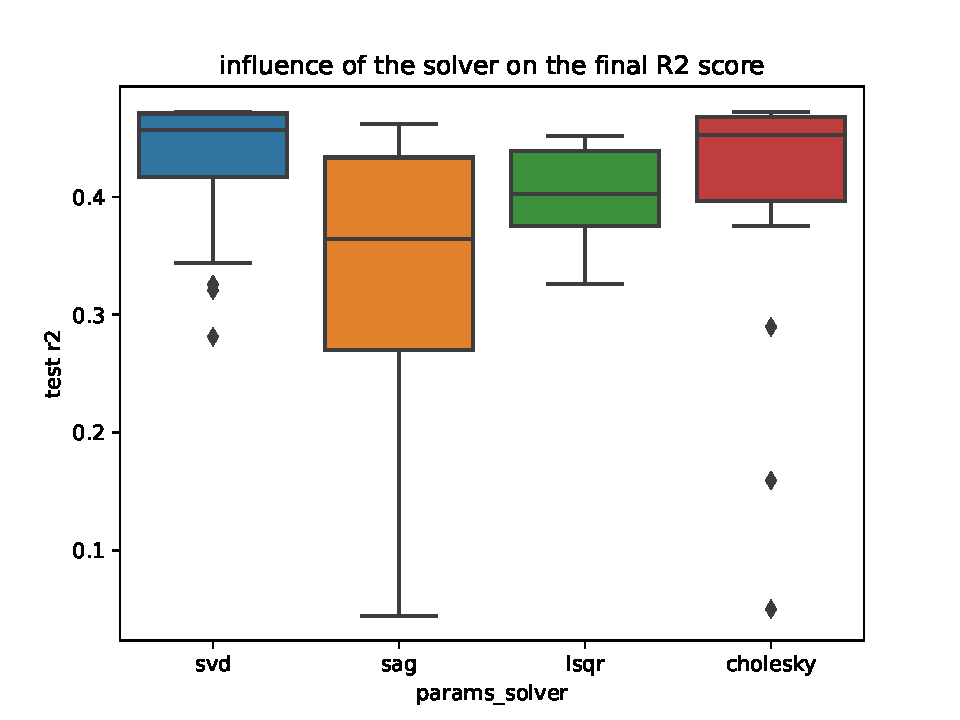
\includegraphics[width=0.8\textwidth]{solver}
        \label{fig:boxplot}
    \end{figure}

\end{frame}

\begin{frame}{Analysis of the hyperparameters}

    \begin{figure}[htpb]
        \centering
        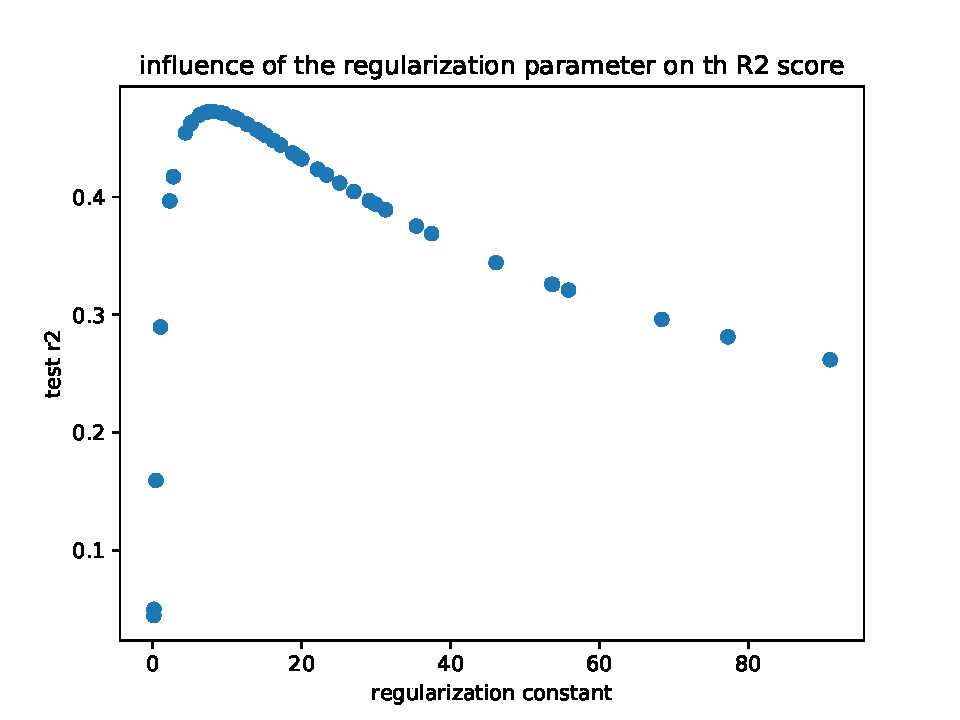
\includegraphics[width=0.8\textwidth]{regularization}
        \label{fig:boxplot}
    \end{figure}

\end{frame}

\begin{frame}{Optuna dashboard}

    \url{https://github.com/optuna/optuna-dashboard} 

    \begin{figure}[htpb]
        \centering
        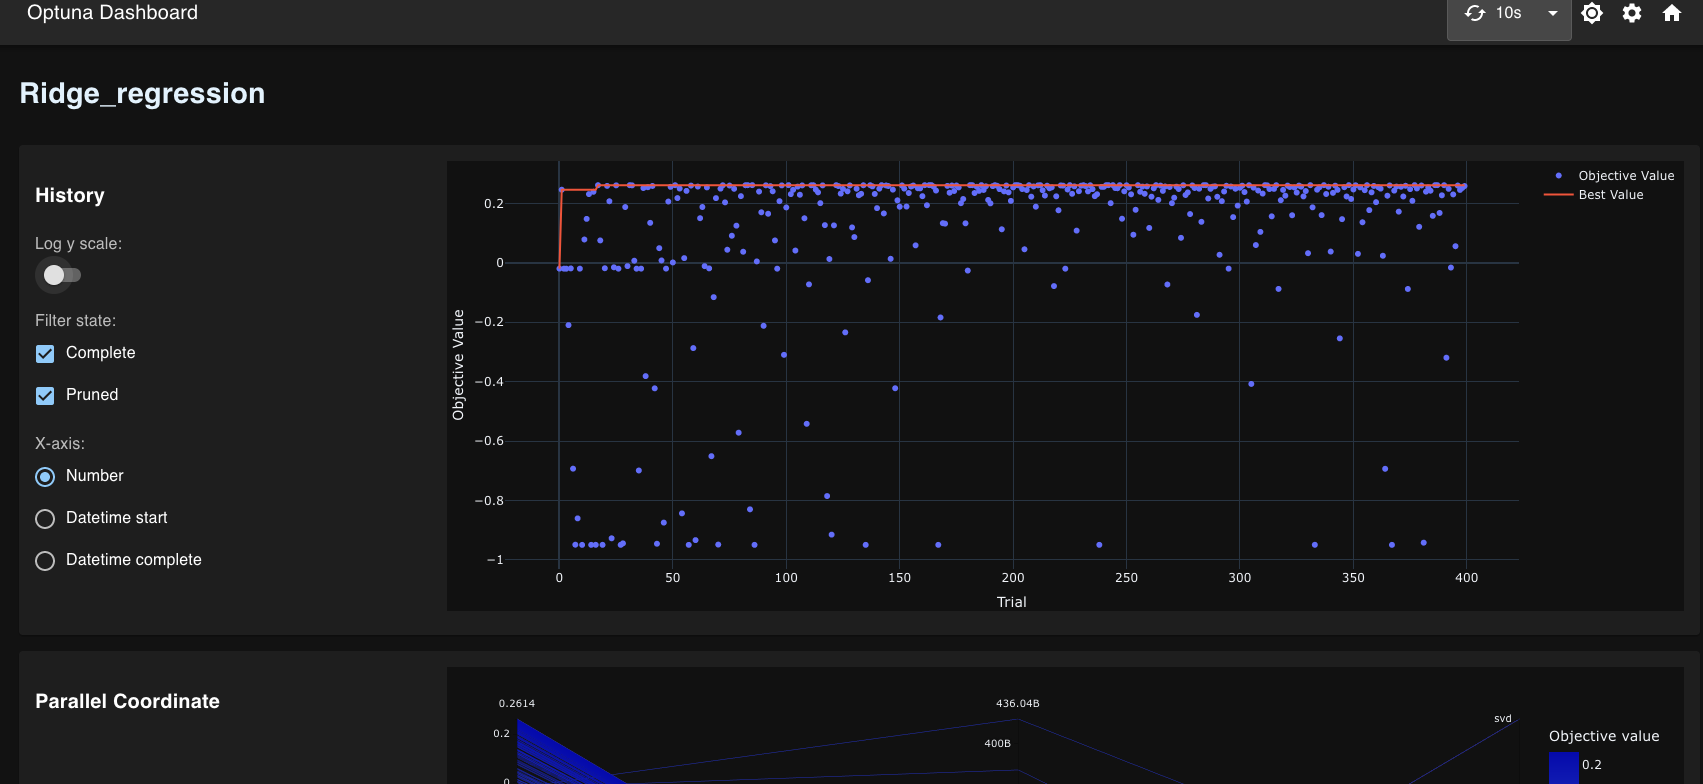
\includegraphics[width=0.8\textwidth]{dashboard}
        \label{fig:dashboard}
    \end{figure}

\end{frame}

\begin{frame}{Multi-objective optimization}

    Optuna can be used to optimize several objectives, e.g.: optimize the score and minimize the computation time (both depend on the hyperparameters).

    Notion of Pareto front.

\end{frame}


\end{document} 
